\chapter{Теория графов}
\section{Основные определения}
Пусть $M$ и $N$ - два конечных множества. Будем называть пару множеств $\langle M, N \rangle$ \textbf{графом}.
При этом элементы множества $M$ называются \textbf{вершинами} графа, элементы множества $N$ - \textbf{дугами} графа. 
Дуга, у которой начало и конец совпадают, называется \textbf{петлей}.
Например, граф с множеством вершин $M = \{A, B, C, D\}$, множеством дуг $N = \{1, 2, 3, 4, 5, 6\}$ и отображением в виде
таблицы, может быть изображен чертежом.

\begin{table}[h]
    % \centering
    \begin{tabular}[c]{ | l | l l l l l l | }
        \hline
        Дуга & 1 & 2 & 3 & 4 & 5 & 6    \\ \hline
        Начало & A & A & A & C & B & D  \\ \hline
        Конец & B & C & D & D & D & B   \\
        \hline
    \end{tabular}
\end{table}

\begin{figure}
    \centering 
    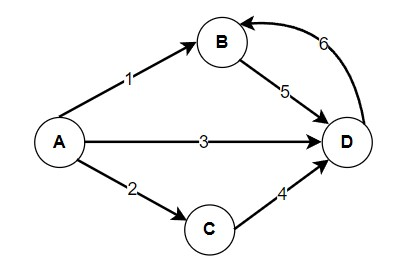
\includegraphics{graph_1.jpg}
    \caption{Пример графа}
\end{figure}
